\section{Spatial Partitioning}
Since in the previous chapter I presented the method for merging 3D Gaussians and outlined some potential issues, the focus of this chapter is to discuss scene partitioning methods, which in the end will be the criterion for selecting groups of primitives for merging. I will first go over two well-known methods in computer graphics that have been explored by other publications on this topic, then present a novel approach and justify its advantages for this application in particular. 

\subsection{Octrees}
Octrees are one of the simplest forms of space partitioning in computer graphics. Usually, the root node of the tree represents the entire axis-aligned bounding box of the model or scene to be partitioned. Then, the node is split into $2 \times 2 \times 2$ nodes, each axis of the box being split simultaneously at its midpoint, resulting in 8 children nodes of equal sizes. The procedure then repeats recursively for all newly generated nodes until a stopping criterion is met. The criterion for stopping the subdivision could be reaching a maximum depth in the tree, reaching a minimum dimension of the leaf nodes, or it could depend on the number of primitives in the leaves since at some point subdividing further would not be beneficial for the application. Every time a node is subdivided, the primitives contained by the parent will be distributed between the children based on the bounding box intersection. Usually, primitives are stored only in the leaf nodes, and the set of primitives contained by an intermediary node can be determined by traversing its subtree. 

The octree can be used either as a structure for partitioning point data, such as vertices in a triangle mesh or a point cloud, or they could be the implicit representation of the data, for cases in which the information is better displayed as voxels than point geometry. Moreover, this kind of structure can be useful for queries in occlusion tests, collision detection or ray tracing.

Being a regular structure, octrees have some advantages. For example, the locations of the splitting planes are predetermined, and the size of the node can be determined during traversal from the size of the root node and the path taken through the tree \cite{RTR4}. However, their regularity comes at a cost if the scene or model does not have a somewhat uniform distribution of primitives inside its bounding box. Since nodes are always generated at half the dimensions of the parent and at predetermined positions, many generated nodes may be empty. Moreover, clusters of very close-by primitives may take a large amount of recursion steps to be split into different nodes, because the splitting planes are generated at specific positions and do not adapt to the data. Figure \ref{fig:octree_diff} shows two examples of octree subdivisions for a set of Gaussians (shown in 2D as a quadtree for easier representation), the illustration on the right highlights the inefficiencies of regular space division, as many nodes end up empty.

\begin{figure}[H]
    \centering
    \includesvg[width=0.9\linewidth]{figures/octree_diff.svg}
    \caption{Octree (quadtree for simplicity) examples for different cases of primitive organization in space. Empty nodes are shown in red.}
    \label{fig:octree_diff}
\end{figure}

To determine the repartition of Gaussians inside nodes, I am using only the center point of the Gaussian, and determining in which one of the eight children each primitive should be distributed. I experimented with considering the bounding box of the confidence ellipsoid and duplicating Gaussians where more nodes overlap, but this leads to an exponential increase of primitives in the acceleration structure. The method I have settled with is using the center point for node assignment and the AABB of the confidence ellipsoids to determine node bounding boxes used in rendering and generating the dynamic LoD. Differences between the node bounds and the computed bounding box for rendering can be seen in Figure \ref{fig:octree_bbox}.

\begin{figure}[H]
    \centering
    \includesvg[width=0.5\linewidth]{figures/octree_bbox.svg}
    \caption{Octree (quadtree for simplicity) showing node bounds and the node AABB computed from confidence ellipsoids.}
    \label{fig:octree_bbox}
\end{figure}

\subsection{BSP Trees}
Binary space partitioning trees are similar to octrees, the main difference being that each node is split into only two child nodes. Also, research on space partitioning for 3DGS suggests that a median split works well for this kind of scene. This approach implies splitting each node along the longest axis of its bounding box. As before, bounding boxes are axis-aligned, just like the splitting planes. To find the splitting plane, all the primitive centers are projected on the longest axis, sorted, and then the median position can be found, through which we will split the node, as shown in figure \ref{fig:bsptree_split}. Then, given that the projected positions are already computed, it is easy to distribute the primitives between the two children. Similarly to the octree, primitives are only stored in the leaf nodes. 

\begin{figure}[H]
    \centering
    \includesvg[width=0.9\linewidth]{figures/split.svg}
    \caption{Node subdivision for BSP tree showing projected centers on the longest axis and the split plane with a red dotted line.}
    \label{fig:bsptree_split}
\end{figure}

Because the positions of the splitting planes are not predetermined, the data structure needs additional storage to hold the information about its volume. On the other side, using a median splitting plane ensures that the final structure is a balanced tree, and there are no empty nodes. Even though BSP trees might need more depth than an octree to partition all primitives, this highly depends on the distribution of the primitives, as can be seen in figure \ref{fig:bsptree_diff}.

\begin{figure}[H]
    \centering
    \includesvg[width=0.9\linewidth]{figures/bsp.svg}
    \caption{BSP tree examples for different cases of primitive organization in space. No empty nodes compared to octree.}
    \label{fig:bsptree_diff}
\end{figure}

Other than the splitting method, for this implementation I am using the same approach as with the octrees, distributing primitives based on center position, and computing an additional bounding box based on the confidence ellipsoid. From my experiments, I have found that using a BSP strategy for generating the LODs gives more natural results since all leaf nodes differ in depth by one at most, so when generating a cut in the tree for creating the appropriate LOD, primitives tend to be more uniformly simplified, instead of having high-frequency Gaussians stuck in higher levels in the tree, which would require more simplification steps to be reached. Also, this structure allows for finer transitions between levels, since only two Gaussians are merged at a time, instead of eight.

\subsection{Hybrid Partitioning}
In this last section, I will present a hybrid space partitioning algorithm that I have implemented for this application, taking into account the advantages and disadvantages observed in the two approaches presented above. This method proved to produce better quality results, which will be discussed in a later chapter.

The first part of this approach involves the initial space subdivision, which is intended to result in a uniform distribution of nodes throughout the scene. Because these nodes are very coarse and contain a high count of primitives, they will not be used for generating the levels of detail. Instead, they are used as a starting point for the second subdivision step. This is why for this initial step I chose to use an octree partitioning approach, up to a specified depth, which is determined usually by the scene complexity.

For the second part of the partitioning, the primitives have to be more carefully grouped into nodes. When generating the LoDs, the distribution of Gaussians in nodes determines the order in which they will be merged, and because there are no further scene optimization steps applied after this, creating quality merged primitives is essential for reliable LoD representation. As discussed above, binary space partitioning is advantageous when considering that the stored Gaussians have to be merged, as we have more flexibility in determining the distribution of primitives in nodes. Moreover, binary splitting allows for finer transitions and more possible intermediate representations, as we have more interior nodes than an octree. 

When merging the primitives as explained in the previous chapter, the best results for merged Gaussians are obtained when the initial primitives have similar properties, whether it is spatial coherency or color similarity. This is because, for Gaussians clustered in space, the resulting distribution will approximate well the volumetric coverage, and for color similarity the resulting color will not deviate too much from the appearance of the initial Gaussians. While the median split method works well in evenly clustering spatial structures, in this implementation I will explore clustering-based methods for distributing Gaussians in the children nodes of the tree.

What I want to achieve in this step of space subdivision is a distribution in which, for a parent that is split into two children, the variance of the primitives inside nodes is low, while the variance between nodes is high. Because both position and color should be taken into consideration, each Gaussian is described by a feature vector $\bm{v} = (x, y, z, r, g, b)$, where the color is taken as the first spherical harmonic coefficient on each channel, as that is the one describing the base color of the primitive, and introducing multiple degrees of the harmonics in the clustering would both be inefficient in terms of computation complexity and would bias the clustering towards color and variations based on viewing position. Also, it is worth mentioning that the position is relative to the node center and normalized to the extent of the node's bounding box, so the clustering would not be biased towards position in large nodes or nodes far from the world origin.

K-means clustering \cite{kmeans} is a very popular clustering algorithm that partitions the observation points in $k$ groups, where $k$ is specified at the beginning. The algorithm is based on a heuristic approach and minimizes within-group variance, which is one of the goals for this step. However, it does not take into account the specific variations of position and color, so these should be first weighted based on their importance in the clustered set. For example, if the spatial distribution is uniform, the clustering should prioritize color, and if the color is uniform the clustering should prioritize spatial features. 

Spectral clustering \cite{spectral} makes use of the eigenvectors of the similarity matrix to project the points in a lower-dimensional space, and the clustering is then performed in this space. This ensures that only the components with the highest observed variation in the dataset are used as a basis for clustering. This method is used widely in graph partitioning, as the similarity matrix is built on the edge costs for traversing the graph. Even without connectivity information, the similarity matrix of a point set can be built based on the Euclidean distance of the feature vectors assigned to the points. While this works for small sets of points, the similarity matrix of $N$ points is of size $N \times N$, and computing its eigenvalues becomes too inefficient for this application considering the amount of Gaussians in the scene. 

DBSCAN \cite{dbscan} is another clustering method that allows partitioning clusters that are not linearly separable, and the point allocation is done through a method similar to region-growing, where points are added to clusters based on the local spatial density. However, this method has the same issue as k-means, where weights for positions and color would have to be computed apriori if we wish to distinguish between features, but an even greater issue is the concept of data noise, which allows this method to leave outliers uncategorized. This does not work for this application, as we wish all the Gaussians to be distributed in a node and take part in the merging process.

Given the insights from these methods, I chose to implement a dimensionality reduction algorithm similar to spectral clustering. However, in order to reduce the computational strain of eigendecomposition for large matrices, I am using the covariance matrix of the feature vectors. Given an intermediary node containing $N$ primitives, we first compute the average feature vector $\bm{\overline{v}}$:
\[
\bm{\overline{v}} = \frac{1}{N} \sum_i^N \bm{v}_i
\]
then the matrix of feature vector variance $D \in \mathbb{R}^{N \times 6}$:
\[
D_i = \bm{v}_i - \bm{\overline{v}}, i \in [1, N] 
\]
and we can obtain the covariance matrix $\Sigma \in \mathbb{R}^{6 \times 6}$ as:
\[
\Sigma = D^T D
\]
Lastly, through eigendecomposition, we obtain the set of six eigenvectors. Let $(\bm{e}_1, \bm{e}_2)$ be the two eigenvectors with the highest associated eigenvalues. This means that the highest amount of variation in the data appears along these two directions. Now, we will project the 6-dimensional data on this 2-dimensional space, resulting in the set of new feature vectors $\bm{u}$:
\[
\bm{u}_i = ((\bm{v}_i - \bm{\overline{v}}) \cdot \bm{e}_1, (\bm{v}_i - \bm{\overline{v}}) \cdot \bm{e}_2) \in \mathbb{R}^2
\]

The last clustering step is to apply k-means on the data points using the new feature vectors to measure point distance and variation from the mean. This method allows us to select the features where the highest variance is observed, automatically bias toward them when clustering, and ideally obtain clearer separation in the new 2-dimensional space. The choice to use only two eigenvectors comes from the fact that we are only clustering the points into two partitions, and using a higher dimensionality did not bring any improvements in my tests. 

To have a visual explanation of this algorithm, figure \ref{fig:cluster_color} shows a set of 2D points with color information, where a cluster of one color is surrounded by points of a different color. These clusters are not linearly separable, so k-means would not be able to determine the clusters by creating a separating plane in the image space. However, after applying the algorithm above, we observe a clear separation of the points, which can then be easily clustered to obtain a better separation. 

\begin{figure}[H]
    \centering
    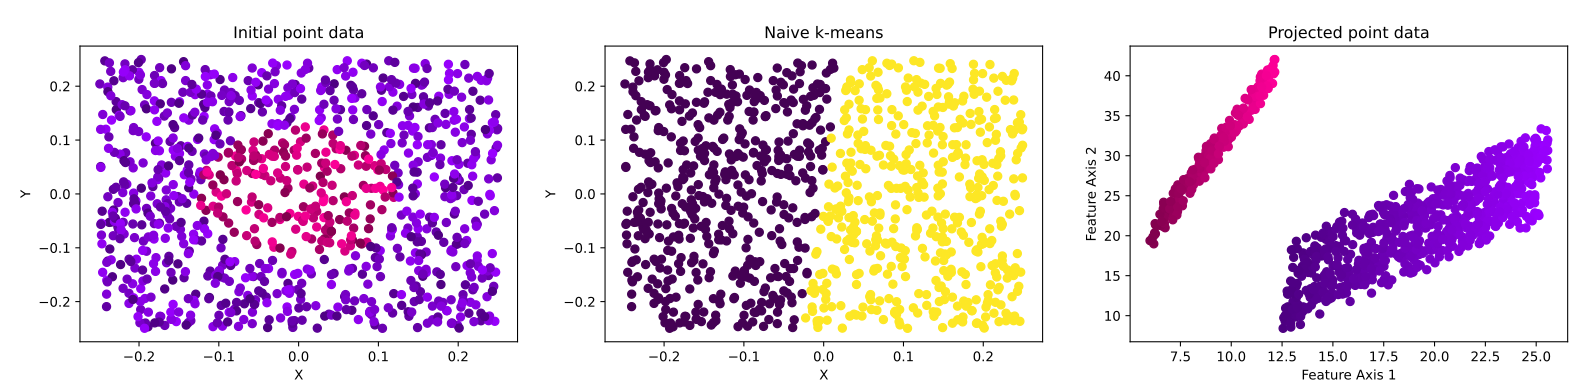
\includegraphics[width=\linewidth]{figures/clustering_color.png}
    \caption{Example of color feature separation in uniform distribution of points in space.}
    \label{fig:cluster_color}
\end{figure}

In order to showcase the spatial feature separation, figure \ref{fig:cluster_space} shows two parallel lines with noise, which are close enough together that k-means would not be able to distinguish between them. However, after projecting to a lower-dimensional space based on feature significance, we get a more distinguished separation. These two cases could be also directly solved by k-means by scaling the data and choosing an appropriate separating axis in the 6-dimensional space, but this algorithm is more robust since the choices for transforming the data are based on the distribution of data in the initial point set. 

\begin{figure}[H]
    \centering
    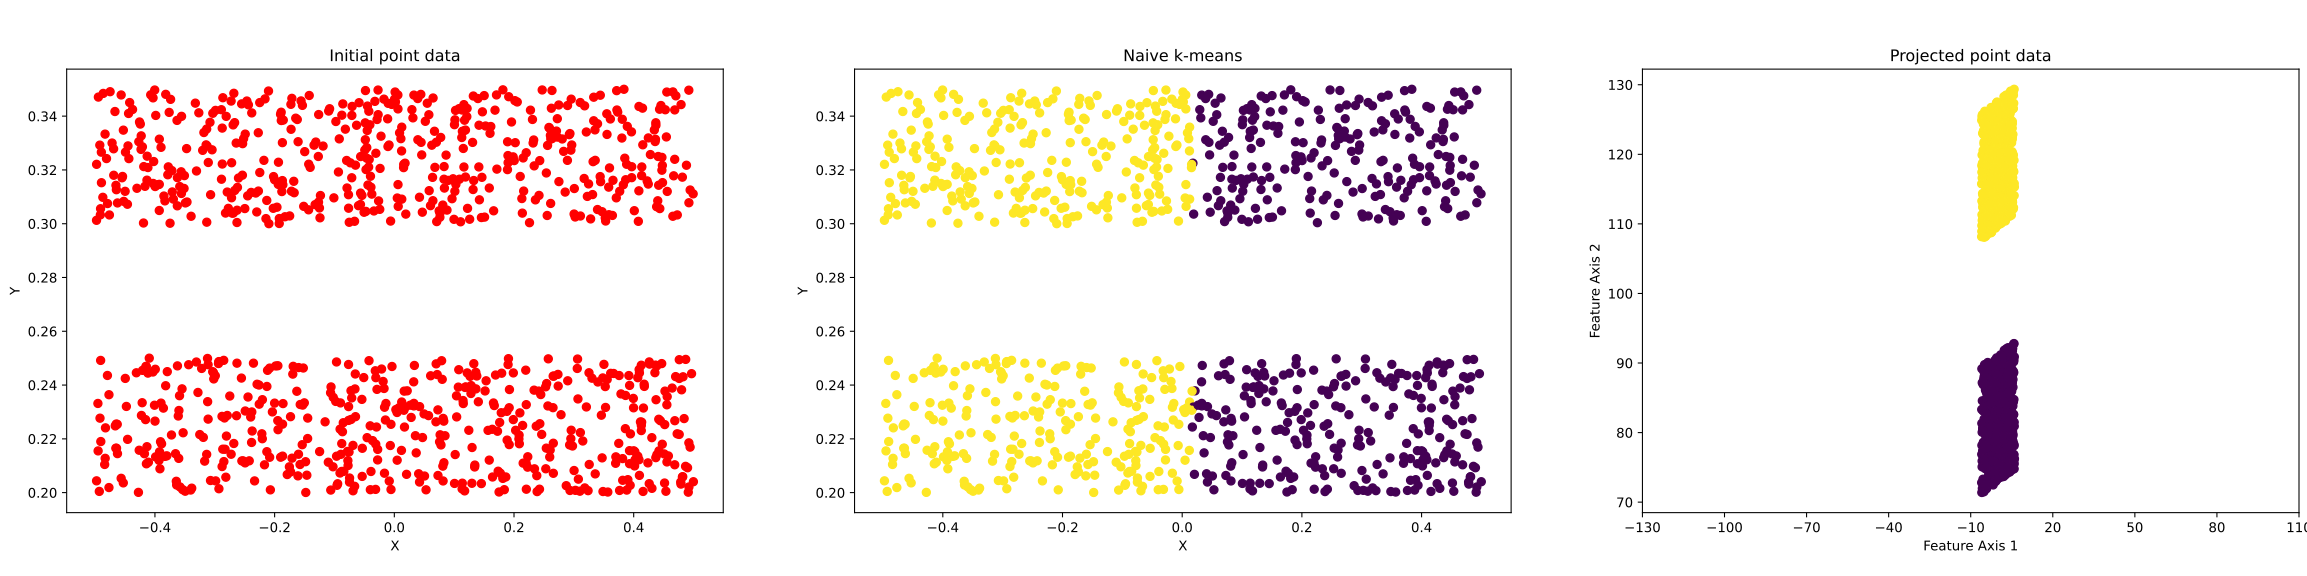
\includegraphics[width=\linewidth]{figures/clustering_space.png}
    \caption{Example of spatial feature separation with uniform color.}
    \label{fig:cluster_space}
\end{figure}

Note that this partitioning approach for the BSP component of the tree does not result in volumetric separation of the primitives, and in some cases, the bounding boxes of the resulting children nodes might have significant overlap. However, this produces significantly better results in terms of image quality. More examples using actual 3DGS scenes will be shown in the Results chapter. 